\section{{\xtype}: Exception Type Recommender}
\label{sec:type}

\begin{figure}[t]
\begin{center}
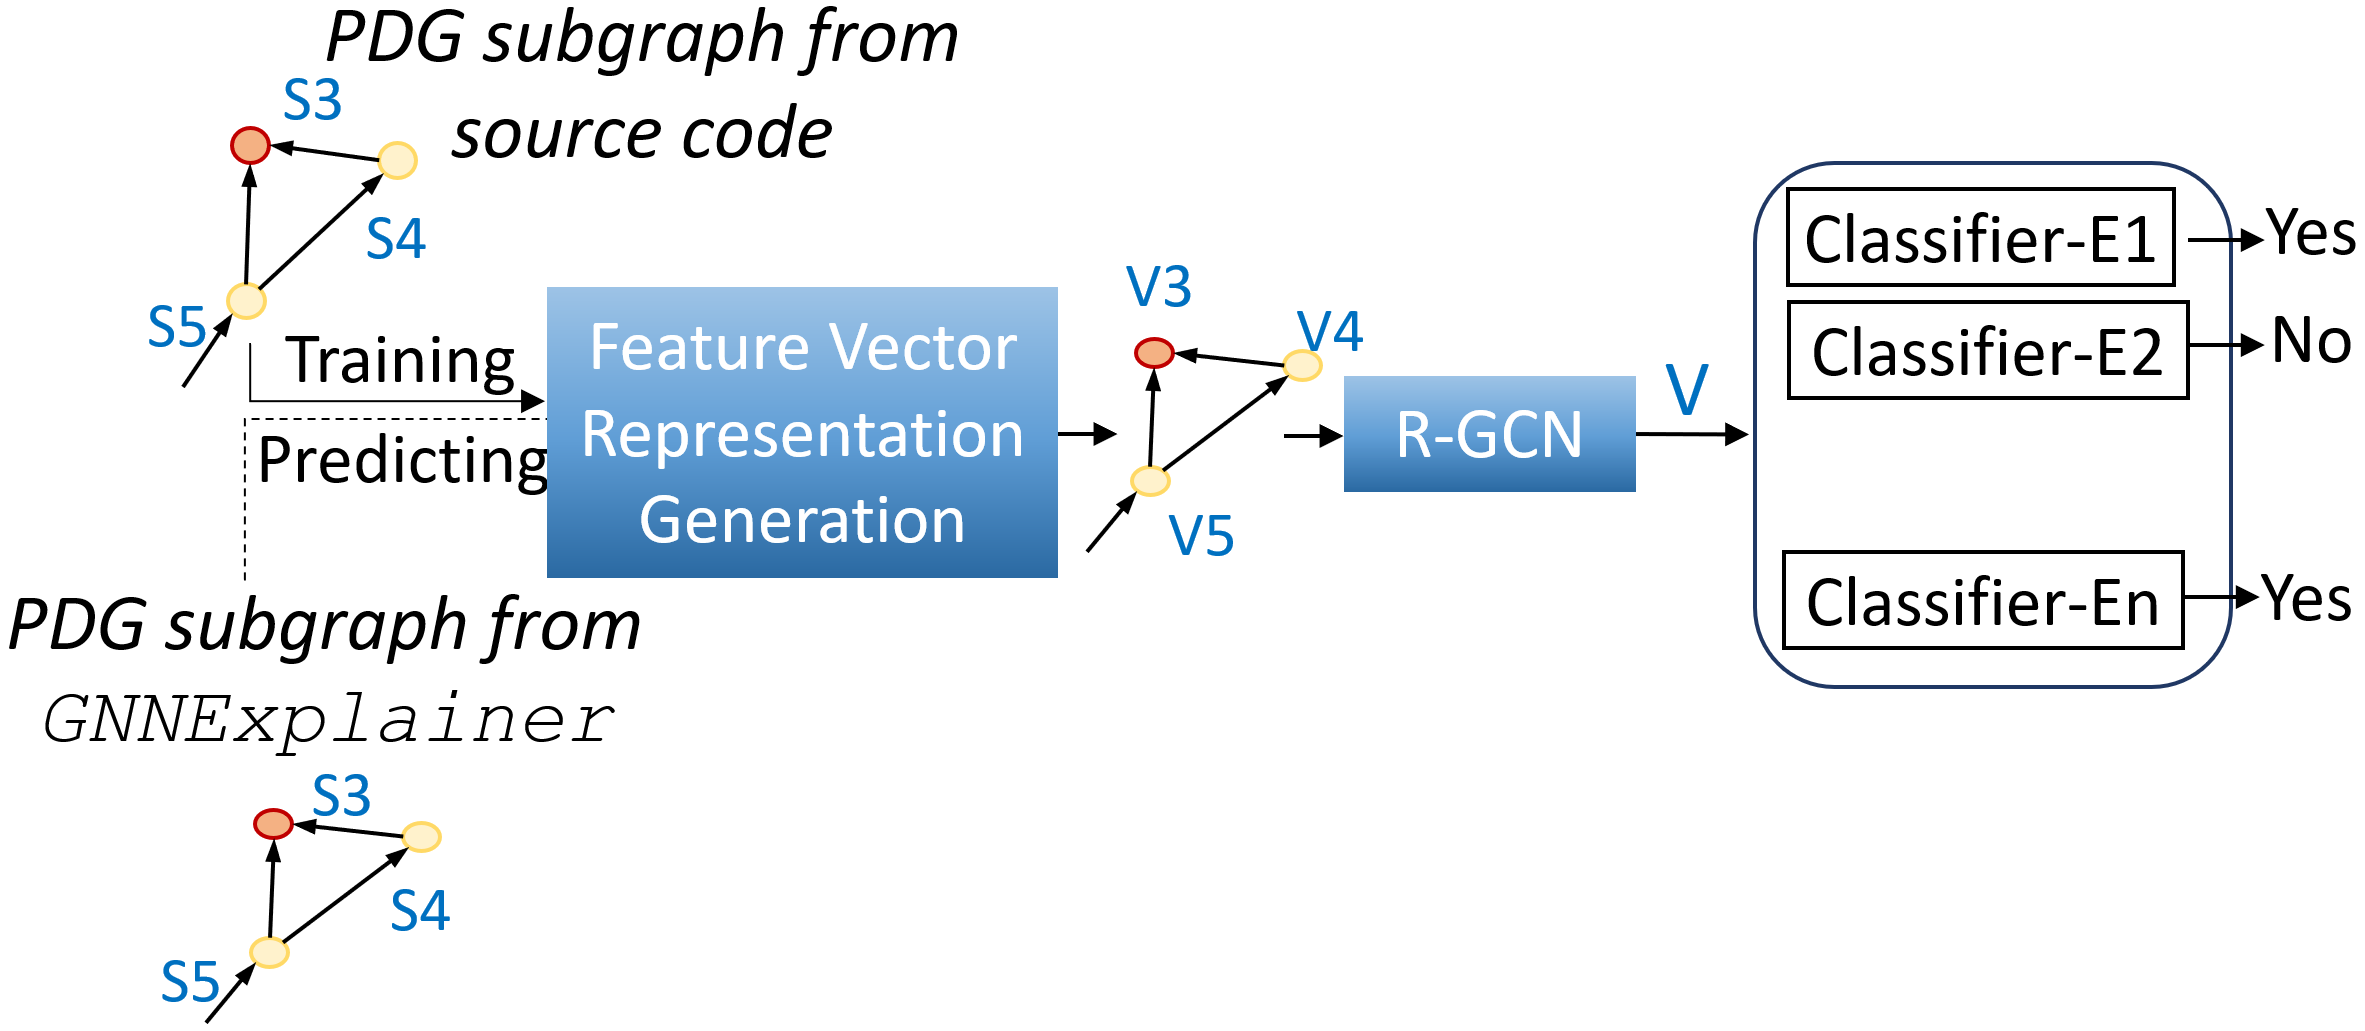
\includegraphics[width=3in]{xtype-3.png}
\vspace{-10pt}
\caption{Exception Type Recommendation ({\xtype})}
\label{fig:xtype}
\end{center}
\end{figure}

This section describes {\xtype} that recommends the exception types to
be handled in the \code{catch} clause for the given code, after the code was
determined to require a \code{try-catch} block and some of its
statements were determined to be placed in the \code{try-catch} block.

We use another R-GCN model that acts as a classifier for different
exception types (Figure~\ref{overview}). For training, the source code
with \code{try-catch} blocks is used as input. {\tool} parses and
processes them in the same way to build the PDG subgraph and the
feature vector representations for the statements as in {\xblock}
(Figure~\ref{fig:feature}). However, in prediction, the input is the
sub-graph $\mathcal{G}_C$ of the PDG because the GNNExplainer already
determined that those statements in that sub-graph need to be placed
in a \code{try-catch} block. In this case, the feature vectors for the
sub-graph are also built in the same way as in
Figure~\ref{fig:feature}. The R-GCN model processes the input
(sub)graph in a similar manner as in Figure~\ref{fig:gcn} except for the
processing on the model's output. Instead of connecting
the output of the R-GCN model to a fully connected layer, we
feed that output to multiple softmax functions to act as the
classifiers for the exception types in the dictionary (e.g.,
\code{IOException}). Each classifier is responsible for one exception
type.  We could set the maximum number of exception types. The
positive output from a classifier indicates the presence of the
corresponding exception type in the \code{catch} clause.
